\documentclass[12pt]{report}
\usepackage{indentfirst}
\usepackage{geometry}
\usepackage{flafter}
\usepackage{graphicx}
\usepackage{float}
\usepackage{titlesec}
\usepackage{tabularx}

\graphicspath{ {.} }
\newgeometry{vmargin={15mm}, hmargin={30mm,30mm}}
\titleformat{\chapter}{\normalfont\huge}{\bf\thechapter.}{18pt}{\huge\bf}

% \title{ \normalsize \textsc{BE PROJECT REPORT}
% 		\\ [2.0cm]
% 		\HRule{0.5pt} \\
% 		\LARGE \textbf{\uppercase{Software Requirements Specification}}
% 		\HRule{2pt} \\ [0.5cm]
% 		\normalsize  \vspace*{5\baselineskip}}

% \date{}

% \author{
% 		Ahmet Eren Çolak - 2587921\\
%         Erdem\\}

\begin{document}

\begin{titlepage}
    \vspace*{4cm}
    \rule{\textwidth}{2px}
    \vspace{0.2cm}
    
    \textbf{\huge{{Software Requirements Specification}}}\par \vspace{0.1cm}
    
    \rule{\textwidth}{2px}
    
    \vspace{1cm}
    
    \begin{tabularx}{\textwidth}{X r}
    \large{Ahmet Eren Çolak }   & \large{Erdem Şamlıoğlu} \\
    2587921 & 2448843
    \end{tabularx}
    
    \vspace{1.3cm}
    
    \vfill
    \today
    
    \end{titlepage}

\tableofcontents
\listoffigures
\listoftables

\chapter{Introduction}

\section{Purpose of the System}
afetbilgi.com is a website created with the aim of providing information and raising awareness 
about natural disasters in Turkey. It was established in response to the lack of easily accessible 
and reliable information during and after disasters. The website provides real-time updates on 
disasters and their impact, as well as information on how to prepare for and respond to emergencies. 
It also offers a platform for individuals and organizations to share their experiences and knowledge, 
creating a community of support and learning. Overall, the project serves as a valuable 
resource for those seeking to stay informed and prepared in the face of natural disasters in Turkey.

\section{Scope}
The afetbilgi.com website will provide essential information on hospitals, assembly points, shelter 
locations, and pharmacies. Users will be able to access information on hospitals and medical centers 
that are available to help earthquake victims. The website will also provide information on designated 
assembly points where people can gather during an emergency. Users will be able to locate shelters 
and other safe locations where they can go during an emergency. Additionally, the website will provide 
information on pharmacies where people can obtain medication and other essential supplies.
\newline

In addition to essential information, afetbilgi.com will also provide supporting information on 
helping centers. The website will provide information on centers that provide assistance and support 
to earthquake victims. Users who want to support earthquake victims will be able to find resources on
how to donate and support relief efforts.
\newline

To make the information more accessible, afetbilgi.com will support multiple languages, including 
Turkish, Kurdish, Arabic, and English. The website will integrate Google Maps to provide users with 
a visual representation of where essential locations are located. Users will be able to filter 
information based on their location to receive the most relevant results. Additionally, the website 
will provide users with the option to download PDFs of the information for offline usage.
\newline

Overall, AfetBilgi.com is designed to be a well-rounded and useful resource for earthquake victims 
and their communities. The website aims to provide a comprehensive collection of information that is 
easy to access and use, with the ultimate goal of helping people during difficult times.

\section{System Overview}

\subsection{System Perspective}

\begin{figure}[H]
    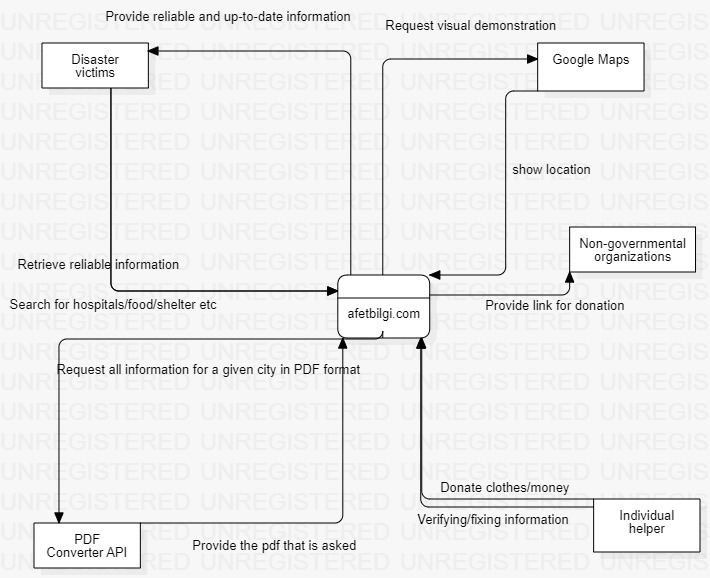
\includegraphics[scale=0.5]{context-diagram}
    \centering
    \caption{Context diagram}
\end{figure}

\subsubsection*{System Interfaces}
Using Google Maps API to show where important information is located. Integration with
social media sites for sharing information. APIs are used for getting data from external 
sources like pharmacies and hospitals.

\subsubsection*{User Interfaces}
User-friendly interface for language and location-based information search with filtering system
for the best viewing experience across many platforms, including desktops, laptops, tablets, and
smartphones, using responsive design. Users have the choice to download reliable information PDFs
for cities for offline use.

\subsubsection*{Software Interfaces}
Using Google Maps API integration to display locations. Information is shared through integration
with social media platforms. PDF Converter API is used to enable users download reliable and up-to-date
information about cities for offline use. Language translation API is used to make website more accessible to 
speakers of other languages.

\subsubsection*{Communication Interfaces}
Provide links for donation and help for individuals/non-governmental organizations. HTTPS protocol 
is used to exchange data with the end-user, including payment and personal information.

\subsubsection*{Memory Constraints}
Since visitors could only have a limited amount of internet connectivity in an emergency, the
website is optimized for quick loading and low bandwidth usage. To ensure that it can be accessible
on low-end devices, the website is built to use the least amount of RAM possible.

\subsubsection*{Operations}
User operations: Search for hospitals, shelter locations, gathering places and pharmacies etc.
View details on pharmacies, hospitals, gathering places, and shelters. Filter the website with one of
the provided languages. Download PDFs

Admin operations: Update the website frequently with the most recent details and information. Create regular
website backups for a server failure.

Overall operations: Maintaining the website often to keep it up-to-date and functional. The website
is optimized for quick loading and low bandwidth usage. Information that is sent by users should
be verified and added to system.


\subsection{System Functions}
\renewcommand{\arraystretch}{2}
\begin{table}[H]
    
    \begin{tabular}{|l|p{10cm}|}
        \hline
    \textbf{Function}              & \textbf{Description} \\ \hline
    View accomodation places       & List possible temporary acommodation places in the selected city \\ \hline
    View gathering places          & List safe gathering places in cities affected from the earthquake \\ \hline
    View evacuation points         & List evacuation points for the selected city \\ \hline
    View transportation aids       & List institutions and their information which provide transportation service for earthquake victims \\ \hline
    View food distribution centers & List available food distribution centers and their information in the selected city \\ \hline
    View gas stations              & List gas station locations in the selected city \\ \hline
    View donation information      & List monetary donation informations, blood donation informations and digital solidarity campaigns \\ \hline
    View health services           & List hospital, pharmacy and veterinerian locations in the selected city \\ \hline
    Filter by city                 & Filter all information by city \\ \hline
    Generate PDF                   & Generate PDF output of helping informations for offline usage \\ \hline
    View on Google Maps            & View locations on the Google Maps \\ \hline
    \end{tabular}
    \caption{System functions}
\end{table}


\subsection{Stakeholder Characteristics}
There are two main users of afetbilgi.com which are users and developers.

Users can be grouped into three: Disaster victims, non-governmental organizations and individual helpers. Users are the ones visiting the website for searching information and resources related to natural disasters in Turkey. 

For disaster victims, they can search the closest shelters, food, hospitals, pharmacies and information gathered by the website. They can use the website to create pdf of information related to the cities and visualize the locations they want. The website is easy to use, therefore disaster victims just need the internet connection to click on the website and use it.

For non-governmental organizations, they can find the donation links and they might use the website to coordinate relief efforts. Therefore, they require technical information about the resources available.

For individual helpers, same with the non-governmental organizations, they can find donation links for money, food and blood. They can also help the developers to verify the information and if something is wrong, they can contact them through the link provided. Just like disaster victims, individual helpers just need the internet connection to use the website.

Developers for afetbilgi.com are responsible for creating, maintaining, updating and verifying the data. They gather all the information they can about the cities especially the cities that has been affected by the disaster and categorize them by city. They use some APIs such as Google Maps and PDF Converter to make users’ lives easier. Developers need to have high computer skills, good coding skills and knowledge about creating websites.

\subsection{Limitations}
\subsubsection{Regulatory policies}
afetbilgi.com should be considered as a website to provide information and guidance in case of a natural disaster. It should be used to gather reliable information.

\subsubsection{Hardware limitations}
During the peak times for the website, in other words disaster times, website speed and performance might go lower because of the processing and power limitations.

\subsubsection{Interface to other applications}
The system should be able to detect whether the user is connecting through computer or smart phone and create the visual for the page layout and screen size accordingly.

\subsubsection{Parallel operation} 
In afetbilgi.com, multiple processes and algorithms may run concurrently to provide up-to-date information. This might result in delays.

\subsubsection{Audit functions} 
afetbilgi.com does not have any audit functions.

\subsubsection{Control functions}
Control functions are determined by the developers and all of them are reachable for only developers, and it requires necessary privileges.

\subsubsection{High-order language requirements} 
React Native programming language and Typescript is used to create and design afetbilgi.com.

\subsubsection{Signal handshake protocols}
The communication between afetbilgi.com and external sources use secure channels such as HTTPS to ensure data privacy. The website follows established web standards.

\subsubsection{Quality requirements} 
afetbilgi.com is designed to provide up-to-date and reliable information. However, sometimes this might be affected by wrong information provided by people.

\subsubsection{Criticality of the application} 
In case of a disaster, breakdown of the server and wrong information can cause some problems. Therefore, these problems should be solved rapidly.

\subsubsection{Safety and security considerations}
Since the website does not ask for any private data, and only direct the user to other links (donations and other websites), developers only need to verify the links that are provided.

\subsubsection{Physical/mental considerations} 
afetbilgi.com is designed to be used easily by all users.

\subsubsection{Limitations that are sourced from other systems}
There is no such limitation.

\section{Definitions}
HTTPS, Hyper Text Transfer Protocol

RAM, Memory

API, Application Programming Interface

\chapter{References}

Alpaylan. (n.d.). GitHub - alpaylan/afetbilgi.com. GitHub. https://github.com/alpaylan/afetbilgi.com

\chapter{Specific Requirements}

\section{External Interfaces}

\begin{figure}[H]
    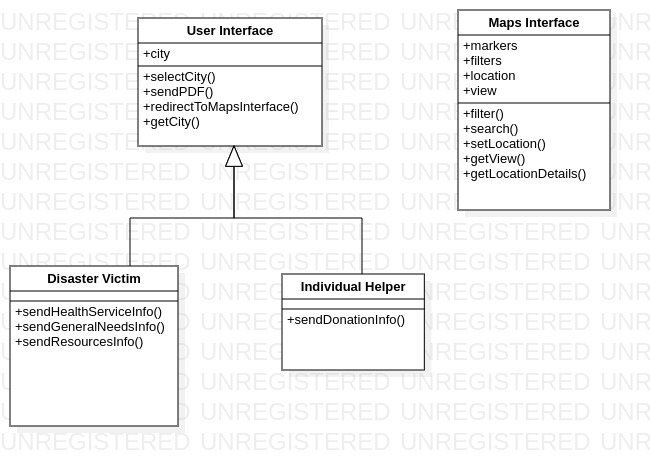
\includegraphics[scale=0.5]{ext1}
    \centering
    \caption{External interfaces}
\end{figure}

\section{Functions}

\begin{figure}[H]
    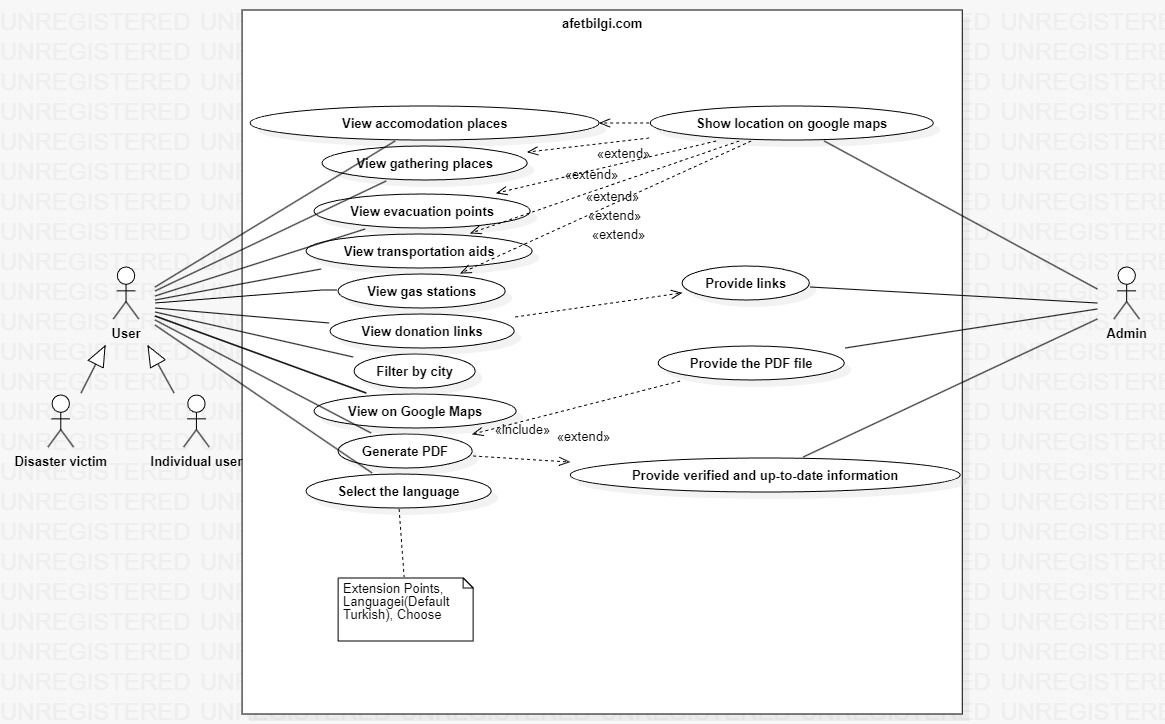
\includegraphics[height=16cm, width=17cm]{use-case}
    \caption{Use-case diagram}
\end{figure}

\vspace*{3cm}
\begin{table}[H]
    \begin{tabular}{|l|p{10cm}|}
    \hline
    \textbf{Use-case Name}    &  View accomodation places \\ \hline
    \textbf{Actors}           &  User \\ \hline
    \textbf{Description}      &  Show a list of available acommodation places nearby\\ \hline
    \textbf{Data}             &  Location of the user \\ \hline
    \textbf{Preconditions}    &  - \\ \hline
    \textbf{Stimulus}         &  Button click \\ \hline
    \textbf{Basic Flow}       &  \begin{tabular}[c]{@{}l@{}} 1. User enters the website \\ 2. User clicks the accomodation places button \\ 3. User selects a location \end{tabular} \\ \hline
    \textbf{Alternative Flow} &  \begin{tabular}[c]{@{}l@{}} 1. User enters the website \\ 2. User filters by location \\ 3. User clicks the accomodation places button  \end{tabular} \\ \hline
    \textbf{Exception Flow}   &  - \\ \hline
    \textbf{Postconditions}   &  User is able to see available acommodation places \\ \hline
    \end{tabular}
    \centering
    \caption{View accomodation places}
\end{table}

\vspace*{3cm}
\begin{table}[H]
    \begin{tabular}{|l|p{10cm}|}
    \hline
    \textbf{Use-case Name}    &  View gathering places \\ \hline
    \textbf{Actors}           &  User \\ \hline
    \textbf{Description}      &  Show a list of available gathering places nearby\\ \hline
    \textbf{Data}             &  Location of the user \\ \hline
    \textbf{Preconditions}    &  - \\ \hline
    \textbf{Stimulus}         &  Button click \\ \hline
    \textbf{Basic Flow}       &  \begin{tabular}[c]{@{}l@{}} 1. User enters the website \\ 2. User clicks the gathering places button \\ 3. User selects a location \end{tabular} \\ \hline
    \textbf{Alternative Flow} &  \begin{tabular}[c]{@{}l@{}} 1. User enters the website \\ 2. User filters by location \\ 3. User clicks the gathering places button  \end{tabular} \\ \hline
    \textbf{Exception Flow}   &  - \\ \hline
    \textbf{Postconditions}   &  User is able to see available gathering places \\ \hline
    \end{tabular}
    \centering
    \caption{View gathering places}
\end{table}

\vspace*{3cm}
\begin{table}[H]
    \begin{tabular}{|l|p{10cm}|}
    \hline
    \textbf{Use-case Name}    &  View evacuation points  \\ \hline
    \textbf{Actors}           &  User \\ \hline
    \textbf{Description}      &  Show a list of evacuation points in a city\\ \hline
    \textbf{Data}             &  Location of the user \\ \hline
    \textbf{Preconditions}    &  - \\ \hline
    \textbf{Stimulus}         &  Button click \\ \hline
    \textbf{Basic Flow}       &  \begin{tabular}[c]{@{}l@{}} 1. User enters the website \\ 2. User clicks the evacuation points button \\ 3. User selects a location \end{tabular} \\ \hline
    \textbf{Alternative Flow} &  \begin{tabular}[c]{@{}l@{}} 1. User enters the website \\ 2. User filters by location \\ 3. User clicks the evacuation points button  \end{tabular} \\ \hline
    \textbf{Exception Flow}   &  - \\ \hline
    \textbf{Postconditions}   &  User is able to see evacuation points in their city \\ \hline
    \end{tabular}
    \centering
    \caption{View evacuation points}
\end{table}

\vspace*{5cm}
\begin{table}[H]
    \begin{tabular}{|l|p{10cm}|}
    \hline
    \textbf{Use-case Name}    &  View transportation aids  \\ \hline
    \textbf{Actors}           &  User \\ \hline
    \textbf{Description}      &  Show a list of transportation aids in the selected city\\ \hline
    \textbf{Data}             &  Location of the user \\ \hline
    \textbf{Preconditions}    &  - \\ \hline
    \textbf{Stimulus}         &  Button click \\ \hline
    \textbf{Basic Flow}       &  \begin{tabular}[c]{@{}l@{}} 1. User enters the website \\ 2. User clicks the transportation aids button \\ 3. User selects a location \end{tabular} \\ \hline
    \textbf{Alternative Flow} &  \begin{tabular}[c]{@{}l@{}} 1. User enters the website \\ 2. User filters by location \\ 3. User clicks the transportation aids button  \end{tabular} \\ \hline
    \textbf{Exception Flow}   &  - \\ \hline
    \textbf{Postconditions}   &  User is able to see transportation aids in their city \\ \hline
    \end{tabular}
    \centering
    \caption{View transportation aids}
\end{table}

\vspace*{5cm}
\begin{table}[H]
    \begin{tabular}{|l|p{10cm}|}
    \hline
    \textbf{Use-case Name}    &  View food distribution centers  \\ \hline
    \textbf{Actors}           &  User \\ \hline
    \textbf{Description}      &  Show a list of food distribution centers in the selected city\\ \hline
    \textbf{Data}             &  Location of the user \\ \hline
    \textbf{Preconditions}    &  - \\ \hline
    \textbf{Stimulus}         &  Button click \\ \hline
    \textbf{Basic Flow}       &  \begin{tabular}[c]{@{}l@{}} 1. User enters the website \\ 2. User clicks the food distribution centers button \\ 3. User selects a location \end{tabular} \\ \hline
    \textbf{Alternative Flow} &  \begin{tabular}[c]{@{}l@{}} 1. User enters the website \\ 2. User filters by location \\ 3. User clicks the food distribution centers button  \end{tabular} \\ \hline
    \textbf{Exception Flow}   &  - \\ \hline
    \textbf{Postconditions}   &  User is able to see food distribution centers in their city \\ \hline
    \end{tabular}
    \centering
    \caption{View food distribution centers}
\end{table}

\vspace*{5cm}
\begin{table}[H]
    \begin{tabular}{|l|p{10cm}|}
    \hline
    \textbf{Use-case Name}    &  View gas stations  \\ \hline
    \textbf{Actors}           &  User \\ \hline
    \textbf{Description}      &  Show a list of gas stations in the selected city\\ \hline
    \textbf{Data}             &  Location of the user \\ \hline
    \textbf{Preconditions}    &  - \\ \hline
    \textbf{Stimulus}         &  Button click \\ \hline
    \textbf{Basic Flow}       &  \begin{tabular}[c]{@{}l@{}} 1. User enters the website \\ 2. User clicks the gas stations button \\ 3. User selects a location \end{tabular} \\ \hline
    \textbf{Alternative Flow} &  \begin{tabular}[c]{@{}l@{}} 1. User enters the website \\ 2. User filters by location \\ 3. User clicks the gas stations button  \end{tabular} \\ \hline
    \textbf{Exception Flow}   &  - \\ \hline
    \textbf{Postconditions}   &  User is able to see gas stations in their city \\ \hline
    \end{tabular}
    \centering
    \caption{View gas stations}
\end{table}

\vspace*{5cm}
\begin{table}[H]
    \begin{tabular}{|l|p{10cm}|}
    \hline
    \textbf{Use-case Name}    &  View donation information  \\ \hline
    \textbf{Actors}           &  User \\ \hline
    \textbf{Description}      &  Show donation information for various organizations \\ \hline
    \textbf{Data}             &  - \\ \hline
    \textbf{Preconditions}    &  - \\ \hline
    \textbf{Stimulus}         &  Button click \\ \hline
    \textbf{Basic Flow}       &  \begin{tabular}[c]{@{}l@{}} 1. User enters the website \\ 2. User clicks one of the donation information buttons \end{tabular} \\ \hline
    \textbf{Alternative Flow} &  - \\ \hline
    \textbf{Exception Flow}   &  - \\ \hline
    \textbf{Postconditions}   &  User is able to see donation informations \\ \hline
    \end{tabular}
    \centering
    \caption{View donation information}
\end{table}

\vspace*{3cm}
\begin{table}[H]
    \begin{tabular}{|l|p{10cm}|}
    \hline
    \textbf{Use-case Name}    &  View health services  \\ \hline
    \textbf{Actors}           &  User \\ \hline
    \textbf{Description}      &  Show a list of hospitals, pharmacies and veterinerians in the selected city \\ \hline
    \textbf{Data}             &  Location of the user \\ \hline
    \textbf{Preconditions}    &  - \\ \hline
    \textbf{Stimulus}         &  Button click \\ \hline
    \textbf{Basic Flow}       &  \begin{tabular}[c]{p{10cm}} 1. User enters the website \\ 2. User clicks the hospitals or pharmacies or veterinerians button \\ 3. User selects a location \end{tabular} \\ \hline
    \textbf{Alternative Flow} &  \begin{tabular}[c]{p{10cm}} 1. User enters the website \\ 2. User filters by location \\ 3. User clicks the hospitals or pharmacies or veterinerians button  \end{tabular} \\ \hline
    \textbf{Exception Flow}   &  - \\ \hline
    \textbf{Postconditions}   &  User is able to see hospitals, pharmacies and veterinerians in their city \\ \hline
    \end{tabular}
    \centering
    \caption{View health services}
\end{table}

\vspace*{5cm}
\begin{table}[H]
    \begin{tabular}{|l|p{10cm}|}
    \hline
    \textbf{Use-case Name}    &  Filter by city \\ \hline
    \textbf{Actors}           &  User \\ \hline
    \textbf{Description}      &  Filter all informations and features by the selected city \\ \hline
    \textbf{Data}             &  Location of the user \\ \hline
    \textbf{Preconditions}    &  - \\ \hline
    \textbf{Stimulus}         &  Selecting a city from the dropdown list \\ \hline
    \textbf{Basic Flow}       &  \begin{tabular}[c]{p{9.5cm}} 1. User enters the website \\ 2. User clicks the dropdown list which is at the top of the page \\ 3. User selects a city from the list \end{tabular} \\ \hline
    \textbf{Alternative Flow} &  - \\ \hline
    \textbf{Exception Flow}   &  - \\ \hline
    \textbf{Postconditions}   &  User is able to see all features which are filtered by a city \\ \hline
    \end{tabular}
    \centering
    \caption{Filter by city}
\end{table}

\vspace*{5cm}
\begin{table}[H]
    \begin{tabular}{|l|p{10cm}|}
    \hline
    \textbf{Use-case Name}    &  Generate PDF \\ \hline
    \textbf{Actors}           &  User \\ \hline
    \textbf{Description}      &  Generate a PDF for selected informations or city \\ \hline
    \textbf{Data}             &  Location of the user \\ \hline
    \textbf{Preconditions}    &  - \\ \hline
    \textbf{Stimulus}         &  Button click \\ \hline
    \textbf{Basic Flow}       &  \begin{tabular}[c]{@{}l@{}} 1. User enters the website \\ 2. User clicks generate PDF button \\ 3. User selects a city from the list \end{tabular} \\ \hline
    \textbf{Alternative Flow} &  - \\ \hline
    \textbf{Exception Flow}   &  - \\ \hline
    \textbf{Postconditions}   &  User is able to view infromations for the selected city on a PDF for offline usage \\ \hline
    \end{tabular}
    \centering
    \caption{Generate PDF}
\end{table}

\vspace*{5cm}
\begin{table}[H]
    \begin{tabular}{|l|p{10cm}|}
    \hline
    \textbf{Use-case Name}    &  View on Google Maps \\ \hline
    \textbf{Actors}           &  User \\ \hline
    \textbf{Description}      &  Show locations on the Google Maps \\ \hline
    \textbf{Data}             &  - \\ \hline
    \textbf{Preconditions}    &  - \\ \hline
    \textbf{Stimulus}         &  Button click \\ \hline
    \textbf{Basic Flow}       &  \begin{tabular}[c]{@{}l@{}} 1. User enters the website \\ 2. User clicks map button \\ 3. User filters location on the map \end{tabular} \\ \hline
    \textbf{Alternative Flow} &  - \\ \hline
    \textbf{Exception Flow}   &  - \\ \hline
    \textbf{Postconditions}   &  User is able to view locations and filter them on Google Maps \\ \hline
    \end{tabular}
    \centering
    \caption{View on Google Maps}
\end{table}

\begin{figure}[H]
    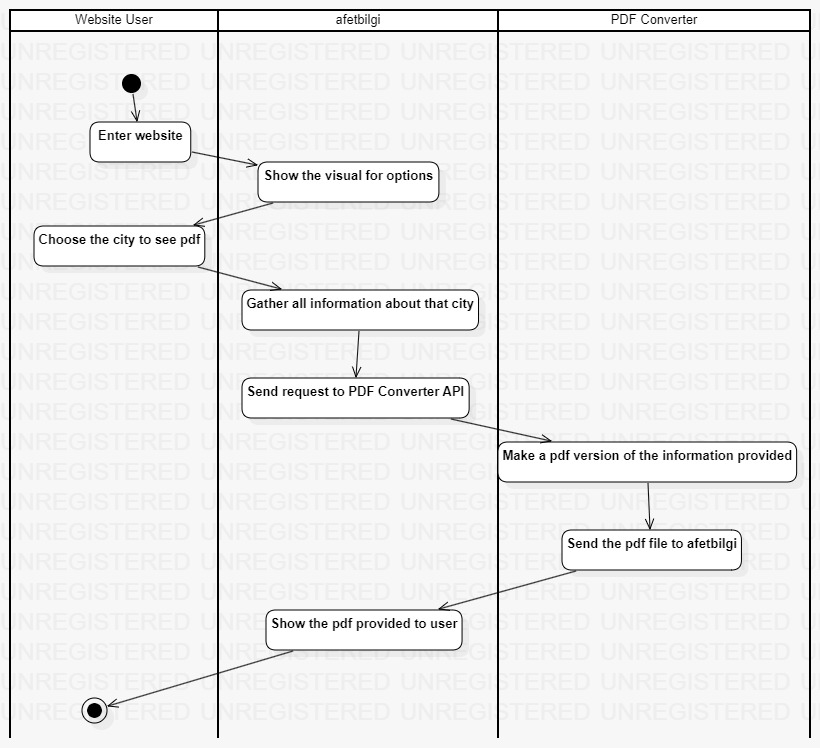
\includegraphics[scale=0.5]{act1}
    \centering
    \caption{Activity diagram}
\end{figure}

\begin{figure}[H]
    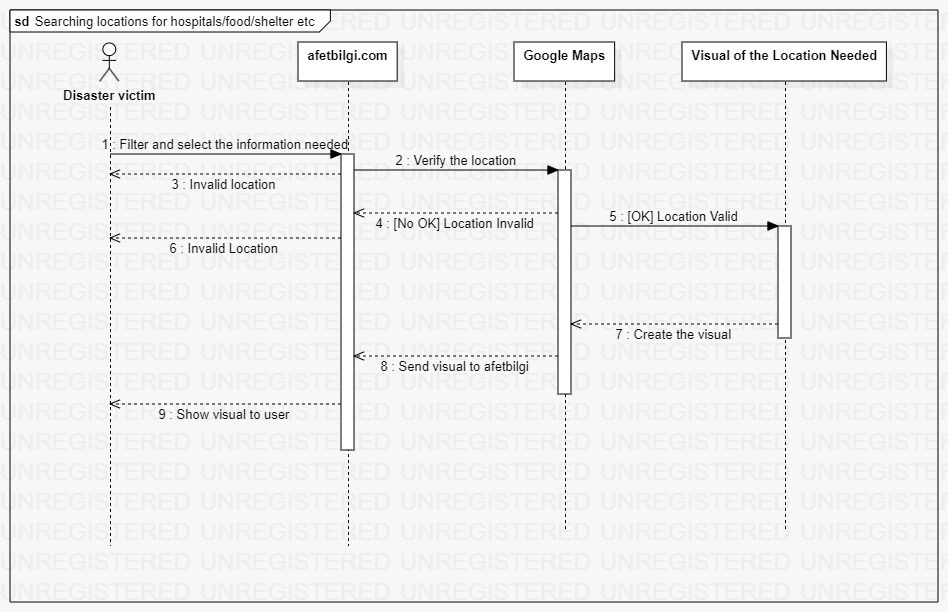
\includegraphics[scale=0.5]{seq1}
    \centering
    \caption{Sequence diagram}
\end{figure}

\begin{figure}[H]
    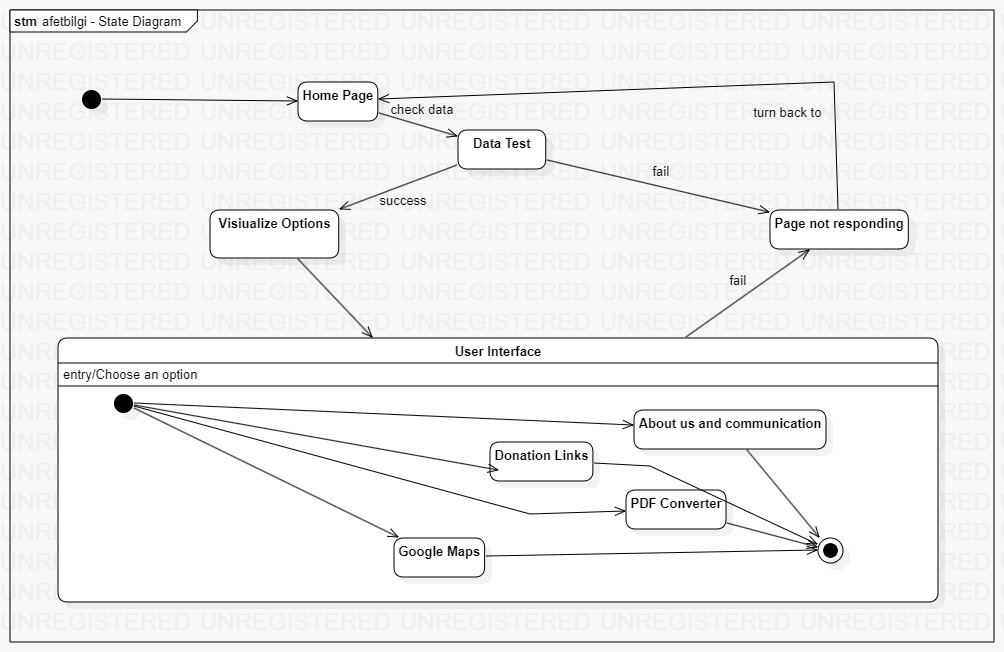
\includegraphics[scale=0.5]{state1}
    \centering
    \caption{State diagram}
\end{figure}

\section{Usability Requirements}
Users should have an internet connection to connect to afetbilgi.com.

Users who have even a slight knowledge about technology shall be able to navigate afetbilgi.com efficiently with basic computer or smartphone or any device that can the access for internet.

Users shall be able to get the information they want about recent and ongoing natural disasters on the homepage in a short time.

Whenever a user wants to find specific information about the disaster, he/she shall be able to find it within at most 3 steps.

Afetbilgi.com shall provide the visual of the location asked or provide the pdf file that is asked.

\section{Performance Requirements}
The system shall be able to handle many users at the same time especially at a disaster time.

All pages and links provided shall be loaded within 3 seconds after a user clicks on them.

Afetbilgi.com shall retrieve the results for any given query in less than 3 seconds.

System shall be able to provide the visual of the location chosen from Google Maps and provide the pdf file that is asked according to the city within 5 seconds at most.

The response time of the database for any operation shall not exceed 10 seconds.

\section{Logical Database Requirements}
\begin{figure}[H]
    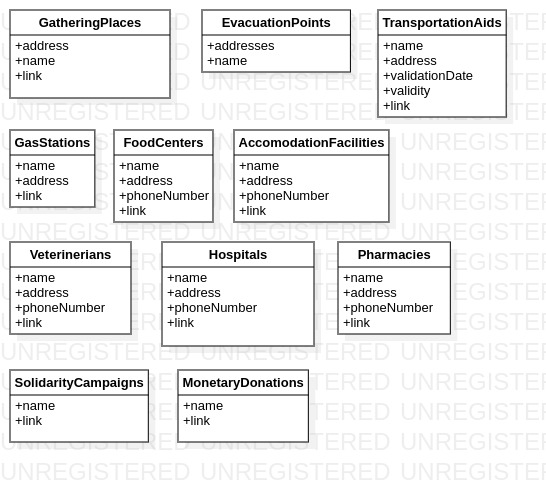
\includegraphics[scale=0.5]{db1}
    \centering
    \caption{Logical Database Diagram}
\end{figure}

The proposed database structure for the emergency information stored on the website involves using separate Google Sheets files to represent tables or collections within the database. Each Google Sheets file would correspond to a separate table/collection in the database, with each row in the file representing a separate record in the table/collection.

The columns in the Google Sheets file would represent the different fields associated with each record, such as the name of the location, its address, phone number, and type of emergency resource it offers. To ensure that the information presented on the website is up-to-date and accurate, the tables/collections would be periodically parsed at specific time intervals.

The parsing process would involve extracting the data from the Google Sheets files, checking for any updates or changes, and then updating the corresponding records in the database accordingly. This approach would provide a simple and efficient way to manage the emergency information stored on the website, as well as enable easy updates to be made by authorized personnel.

The database would be designed to handle a large amount of data, with appropriate indexing and optimization techniques employed to ensure fast and efficient data retrieval. The database would also be secure, with appropriate access controls and permissions put in place to restrict unauthorized access to the data. Finally, the database would be scalable, allowing for additional emergency information to be easily added in the future as needed

\section{Design Constraints}
The website design should be accessible and easy to use for people.

The website should be reachable on multiple devices such as computers, smart phones and basically devices that have access to internet.

The website developers must ensure that the provided links in homepage must be secure links.

The website should support the languages that are spoken in Turkey such as Turkish, English, Kurdish and Arabic.

The website should be optimized for faster loading times.

\section{System Attributes}
\subsubsection{Reliability}
The system shall be able to operate without significant errors or crashes most of the time.
In case of hardware or software failures, the system shall recover automatically.
Data that is stored by the system shall be backed up regularly.
Data that is used by the system should be verified regularly.

\subsubsection{Availability}
The system shall be available 24/7 especially at the disaster times. 
Assuming the device has a stable internet connection, the system shall be available to use within a short time.

\subsubsection{Security}
All links provided on afetbilgi.com must be safe and verified and should not lead to any malicious websites.
The system shall use HTTPS encryption to ensure user data transmitted over the internet is safe.
The website should have protocols to ensure that it is safe from cyber-attacks.

\subsubsection{Maintainability}
The system shall be easily maintainable for developers.
New features or improvements shall be easily implementable to the system without causing any problems.
The system shall require minimal dependency on specific hardware.

\subsubsection{Portability}
The website should be accessible on multiple web browsers, Google Chrome, Opera, Mozilla Firefox, Microsoft Edge etc.
The website shall be able to visualize the pages according to the devices that have different screen sizes.
The database of the server should be easily transferable.

\section{Supporting Information}
afetbilgi.com is a website that was created and designed by volunteers.  A user can use it to search for information, location or get the pdf file of the 
information for cities. Furthermore, users with technical background or have an idea to improve it can contribute to the website by contacting the 
developers through “About us” at homepage of the website. 

\chapter{Suggestions to Improve the System}

\section{System Perspective}
\begin{figure}[H]
    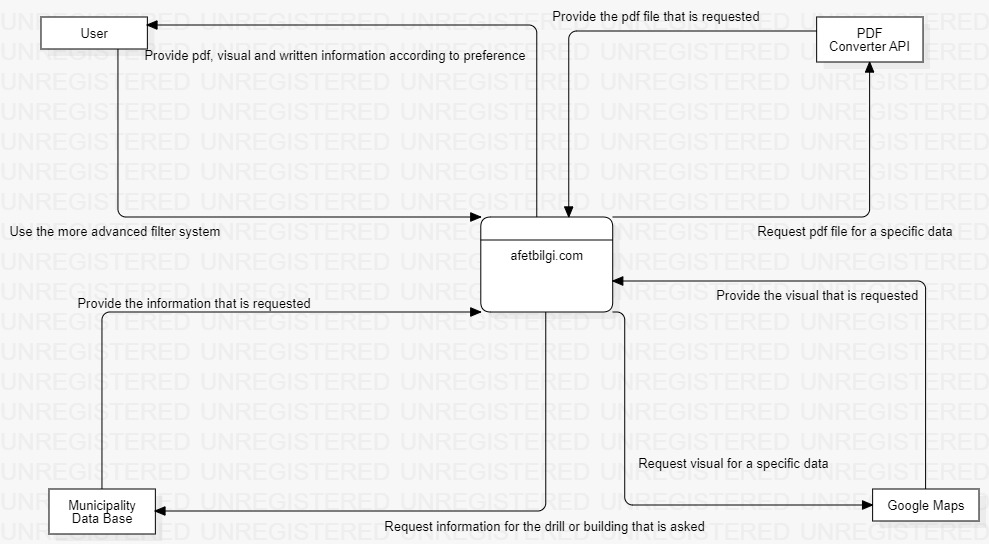
\includegraphics[scale=0.5]{context2}
    \centering
    \caption{Context Diagram Suggestion}
\end{figure}

\subsubsection{System Interfaces}
Using Google Maps, PDF Converter API and Municipality Data Base to provide related and up-to-date information. APIs are also used for getting data from external sources.

\subsubsection{User Interfaces}
Easier to use and find the related information with advanced filter system so that they can reach or get the pdf file also for specific information. Regulating the screen size according to the device that is connected to the server. Users can use pdf files offline too. Users can also upload data to the system and wait for its verification.

\subsubsection{Software Interfaces}
Using Google Maps API integration to visualize the locations according to the search of the user. PDF Converter API is used to give the pdf file that user asked information with filter. REST API to provide information through the website of Municipality.

\subsubsection{Communication Interfaces}
Provide links for donations and help for individuals/non-governmental organizations. HTTPS protocol is used to exchange data with the end-user, including payment and personal information.

\subsubsection{Memory Constraints}
Memory Constraints Since visitors could only have a limited amount of internet connectivity in an emergency, the website is optimized for quick loading and low bandwidth usage. To ensure that it can be accessible on low-end devices, the website is built to use the least amount of RAM possible.

\subsubsection{Operations}
User operations: Use the advanced filter to search for specific information and get the pdf file for it. Upload data and wait for its verification.

Admin operations: Update the website frequently with the most recent details and information. Create regular website backups for a server failure. Check for the data that is uploaded by users and verify it.

Overall operations: Maintaining the website often to keep it up-to-date and functional. The website is optimized for quick loading and low bandwidth usage. Information that is sent by users should be verified and added to the system.

\section{External Interfaces}
\begin{figure}[H]
    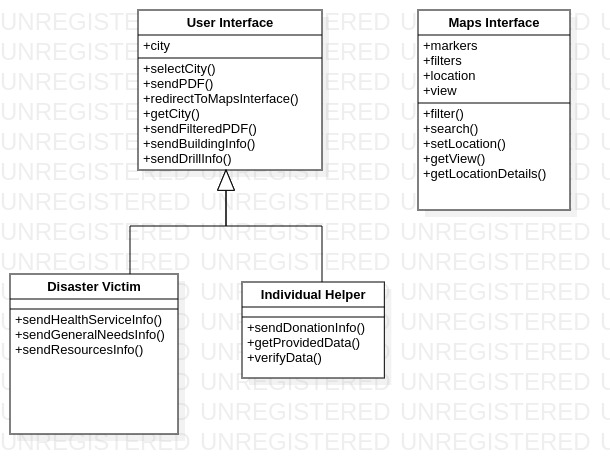
\includegraphics[scale=0.5]{ext2}
    \centering
    \caption{External interfaces suggestion}
\end{figure}

\section{Functions}

\begin{figure}[H]
    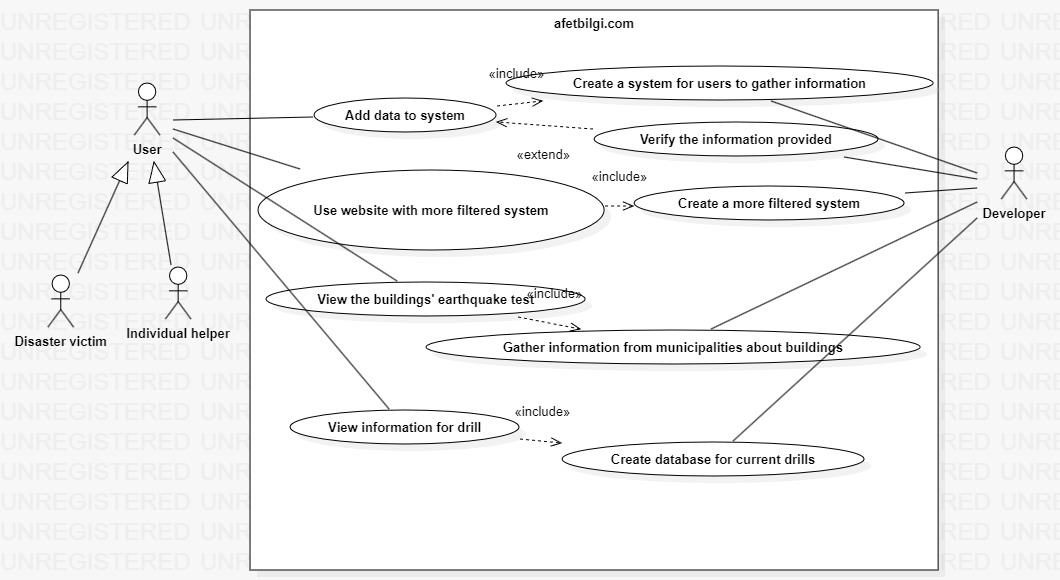
\includegraphics[width=17cm, height=13cm]{use-case2}
    \centering
    \caption{Use-case diagram suggestion}
\end{figure}

\vspace*{5cm}
\begin{table}[H]
    \begin{tabular}{|l|p{10cm}|}
    \hline
    \textbf{Use-case Name}    &  Provide data \\ \hline
    \textbf{Actors}           &  User \\ \hline
    \textbf{Description}      &  Provide helpful data for disaster victims. These data includes types of food centers, acommodation facilities, transportation help, services\\ \hline
    \textbf{Data}             &  Any type of data user wishes to provide\\ \hline
    \textbf{Preconditions}    &  - \\ \hline
    \textbf{Stimulus}         &  Button click \\ \hline
    \textbf{Basic Flow}       &  \begin{tabular}[c]{p{9.5cm}} 1. User enters the website \\ 2. User clicks provide data button \\ 3. User selects data type he wishes to provide (accomodation, transportation, food center, ...) \\ 4. User enters data to text field \\ 5. User clicks send data request \end{tabular} \\ \hline
    \textbf{Alternative Flow} &  - \\ \hline
    \textbf{Exception Flow}   &  - \\ \hline
    \textbf{Postconditions}   &  User is provided his data and waiting for approval of system admins \\ \hline
    \end{tabular}
    \centering
    \caption{Provide data}
\end{table}

\begin{table}[H]
    \begin{tabular}{|l|p{10cm}|}
    \hline
    \textbf{Use-case Name}    &  Generate PDF with filtering\\ \hline
    \textbf{Actors}           &  User \\ \hline
    \textbf{Description}      &  Generate PDF which only includes data which is related to selected filters \\ \hline
    \textbf{Data}             &  Location of the user, filters \\ \hline
    \textbf{Preconditions}    &  - \\ \hline
    \textbf{Stimulus}         &  Button click \\ \hline
    \textbf{Basic Flow}       &  \begin{tabular}[c]{p{9.5cm}} 1. User enters the website \\ 2. User clicks generate PDF button \\ 3. User selects the filters (location, food centers, assembly points, acommodation, ...) \\ 4. User clicks download PDF button \end{tabular} \\ \hline
    \textbf{Alternative Flow} &  - \\ \hline
    \textbf{Exception Flow}   &  - \\ \hline
    \textbf{Postconditions}   &  User is able to read informations which only he requested offline \\ \hline
    \end{tabular}
    \centering
    \caption{Generate PDF with filtering}
\end{table}

\begin{table}[H]
    \begin{tabular}{|l|p{10cm}|}
    \hline
    \textbf{Use-case Name}    &  View disaster drill dates, locations and education centers \\ \hline
    \textbf{Actors}           &  User \\ \hline
    \textbf{Description}      &  Show date and location of disaster drills and education centers in the selected city \\ \hline
    \textbf{Data}             &  Location of the user \\ \hline
    \textbf{Preconditions}    &  - \\ \hline
    \textbf{Stimulus}         &  Button click \\ \hline
    \textbf{Basic Flow}       &  \begin{tabular}[c]{@{}l@{}} 1. User enters the website \\ 2. User clicks view drill and education centers button \\ 3. User selects a city from the list \end{tabular} \\ \hline
    \textbf{Alternative Flow} &  - \\ \hline
    \textbf{Exception Flow}   &  If user filled address form incorrectly then the building will not be found on the database. \\ \hline
    \textbf{Postconditions}   &  User is able to view disaster drill dates, locations and education centers \\ \hline
    \end{tabular}
    \centering
    \caption{View disaster drill dates, locations and education centers}
\end{table}

\begin{table}[H]
    \begin{tabular}{|l|p{10cm}|}
    \hline
    \textbf{Use-case Name}    &  Check building strength \\ \hline
    \textbf{Actors}           &  User \\ \hline
    \textbf{Description}      &  Provide information about a building's strength and status \\ \hline
    \textbf{Data}             &  Address of the building \\ \hline
    \textbf{Preconditions}    &  - \\ \hline
    \textbf{Stimulus}         &  Button click \\ \hline
    \textbf{Basic Flow}       &  \begin{tabular}[c]{@{}l@{}} 1. User enters the website \\ 2. User clicks check building status button \\ 3. User fills the address form \\ 4. User clicks check buildings button \end{tabular} \\ \hline
    \textbf{Alternative Flow} &  - \\ \hline
    \textbf{Postconditions}   &  User is able to view disaster drill dates, locations and education centers \\ \hline
    \end{tabular}
    \centering
    \caption{Check building strength}
\end{table}

\begin{figure}[H]
    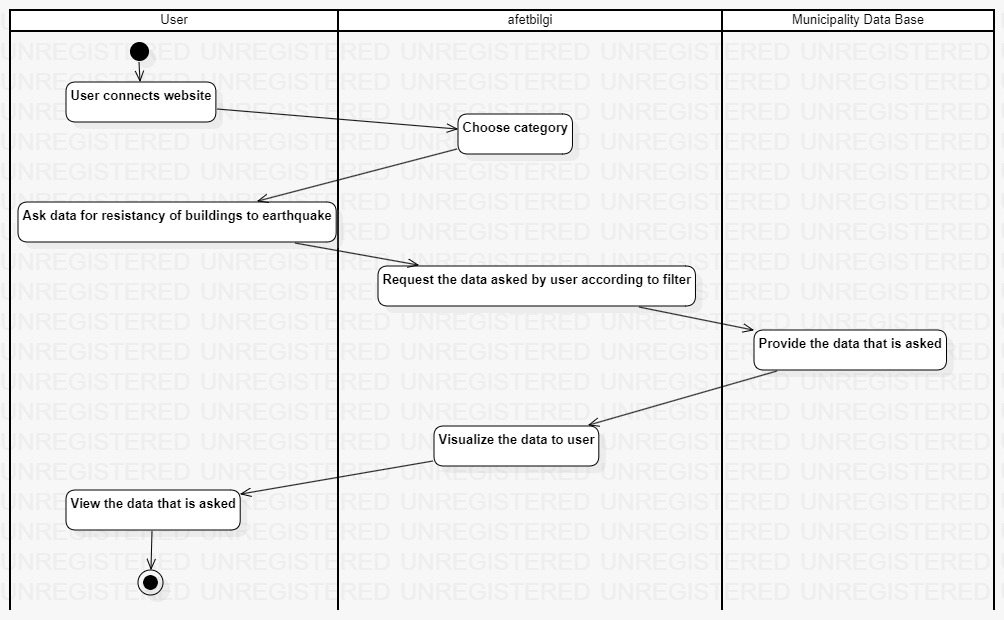
\includegraphics[scale=0.5]{act2}
    \centering
    \caption{Activity diagram suggestion}
\end{figure}

\begin{figure}[H]
    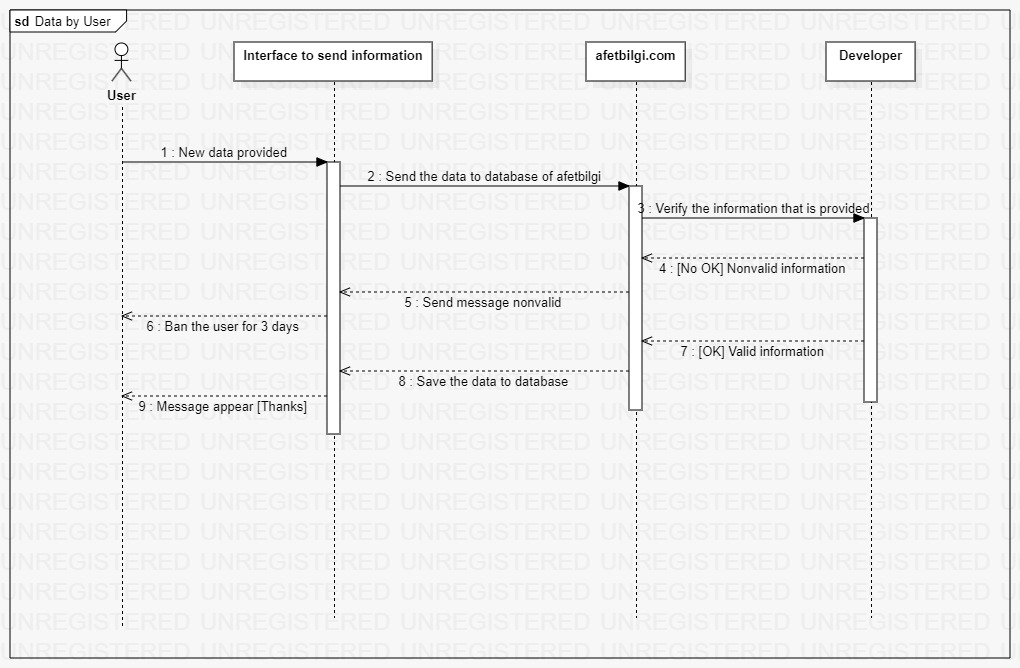
\includegraphics[scale=0.5]{seq2}
    \centering
    \caption{Sequence diagram suggestion}
\end{figure}

\begin{figure}[H]
    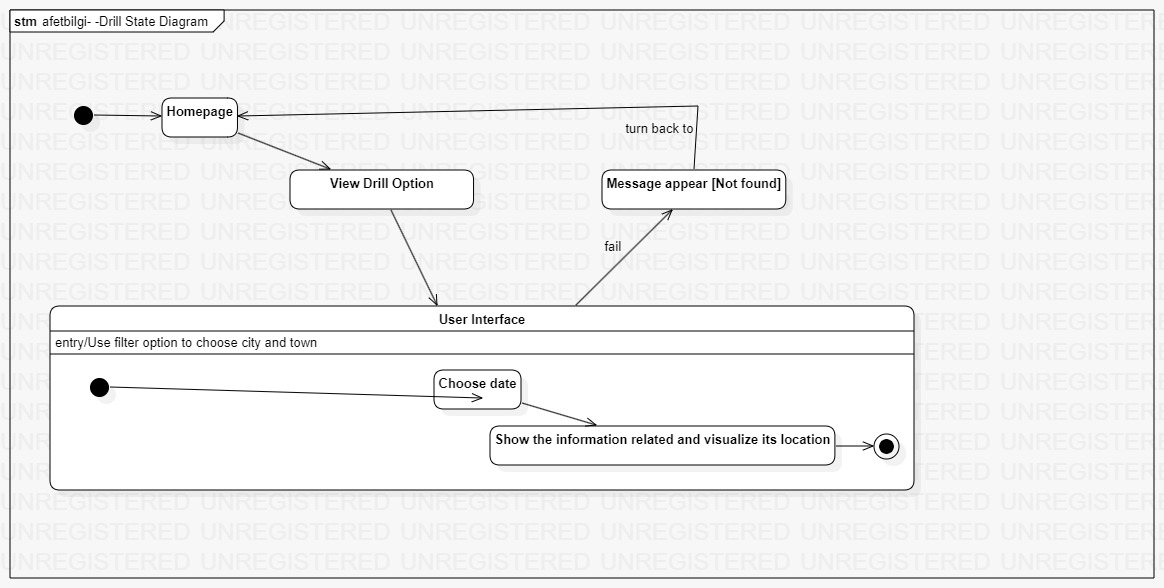
\includegraphics[scale=0.5]{state2}
    \centering
    \caption{State diagram suggestion}
\end{figure}

\section{Usability Requirements}
Users still need an internet connection to benefit from these new features.

User should select and specify related filters for advanced PDF generation.

Users should provide exact address and location for buildings which they are willing to learn about their strength against disasters.

Users should specify their location to learn about disaster drill and education locations and dates.

\section{Performance Requirements}System Interfaces
Using Google Maps, PDF Converter API and Municipality Data Base to provide related and up-to-date information. APIs are also used for getting data from external sources.

User Interfaces
Easier to use and find the related information with advanced filter system so that they can reach or get the pdf file also for specific information. Regulating the screen size according to the device that is connected to the server. Users can use pdf files offline too. Users can also upload data to the system and wait for its verification.

Software Interfaces
Using Google Maps API integration to visualize the locations according to the search of the user. PDF Converter API is used to give the pdf file that user asked information with filter. REST API to provide information through the website of Municipality.

Communication Interfaces
Provide links for donations and help for individuals/non-governmental organizations. HTTPS protocol is used to exchange data with the end-user, including payment and personal information.

Memory Constraints
Memory Constraints Since visitors could only have a limited amount of internet connectivity in an emergency, the website is optimized for quick loading and low bandwidth usage. To ensure that it can be accessible on low-end devices, the website is built to use the least amount of RAM possible.

Operations
User operations: Use the advanced filter to search for specific information and get the pdf file for it. Upload data and wait for its verification.
Admin operations: Update the website frequently with the most recent details and information. Create regular website backups for a server failure. Check for the data that is uploaded by users and verify it.
Overall operations: Maintaining the website often to keep it up-to-date and functional. The website is optimized for quick loading and low bandwidth usage. Information that is sent by users should be verified and added to the system.
The website should quickly generate the PDF with the contents which user asked to and respond to user in an efficient way.

Data which an individual helper wants to share with the website, should be verified quickly by system admins and put into the database of the website.

Website should quickly retrieve information from the municipalities' database about the building which user asked to find out about its strength against earthquakes.

\section{Logical Database Requirements}
\begin{figure}[H]
    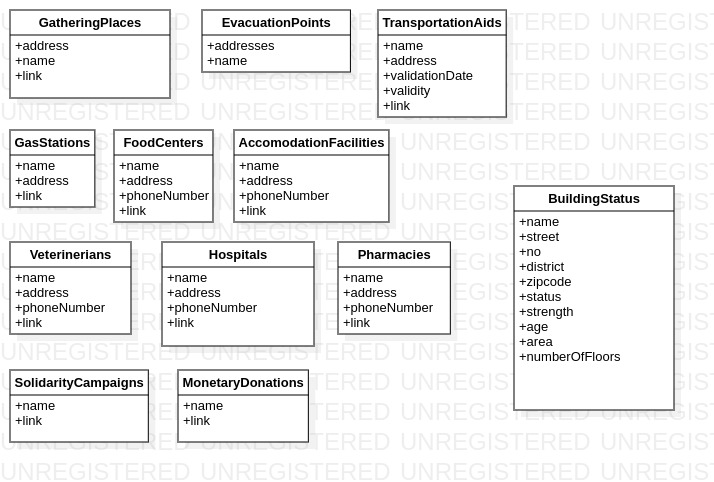
\includegraphics[scale=0.5]{db2}
    \centering
    \caption{Logical Database Diagram Suggestion}
\end{figure}

\section{Design Constraints}
System admins should regularly verify and update the website as users share useful and up-to-date data about disasters.

Address specification for buildings' strength information should be easy to understand and descriptive for users.

Filter options for advanced PDF generation must be clear and easy to use for users.


\section{System Attributes}

\subsubsection{Reliability}
Data provided by individual helpers should be carefully inspected and verified by system admins. These data also must be backed up in case of any failure of the system.

PDF generation with filters should not include irrelevant information. Filters must work properly.

\subsubsection{Availability}
Assuming user has a stable internet connection, user must be able benefit from PDF generation with filters, building strength checking, disaster drill and education information and sata sharing features all the time.
All these features must be available in all kinds of browsers.

\subsubsection{Security}
For retrieving building informations, connection between municipalities' databases and afetbilgi.com should be secure and reliable so that any possible attack must not succeed.

\subsubsection{Maintainability}
Newly added features should be implemented in a way such that it is easy to change, update and develop on top of for the developers of the system.

\section{Supporting Information}
The aim of the four features proposed is to enhance the website's functionality and usefulness, providing users with advanced tools and 
resources to help them prepare for and respond to emergency situations. These features aim to provide users with customized information, 
enable user sharing and verification of information, provide accurate information on building status and strength, and offer information on 
upcoming disaster drills and training sessions. Ultimately, these features aim to promote safety and resilience in the face of natural disasters.

\end{document}